%! Author = Yilin
%! Date = 2025/1/26

Despite the continuous evolution of national cybercrime since the inception of data collection,
along with changes in policies, legal frameworks, and population demographics,
we can create a global cybercrime hotspot map by leveraging crime data recorded by VERIS over the years.
This not only facilitates the analysis of cybercrime volumes by country
but also allows for fitting the data against policy and population variables to assess their influence on cybercrime trends.
\subsection{Cybercrime distribution across the globe}\label{subsec:building-the-hotspot-map} %3.1
	We made use of a world-wide map to represent all cybercrime occurred around the world.
	In the map, the color filled in each country represents the total number of cybercrime incidents recorded since the beginning of the statistics.
	The color gradient, ranging from dark blue to dark red, corresponds to eight severity levels (1 to 8).
	Countries marked in blue indicate a low frequency of cybercrime incidents, while those marked in red represent a high density of such incidents.
	For instance, the United States, where the VERIS concept was first proposed, has the highest number of recorded incidents (7,236),
	whereas many other countries have only 1 or 2 recorded incidents.
	To address this significant disparity in data distribution, we applied a logarithmic transformation to the data using the formula
	\[ y=\log(1+x) \]
	where x here represents $D_i$.
	This transformation was implemented using the function
	\[ np.log1p() \]
	in Python to ensure computational precision and stability, particularly for small values.
	The final results are visualized in Figure 1.
	\begin{figure}[htbp]
		\centering
		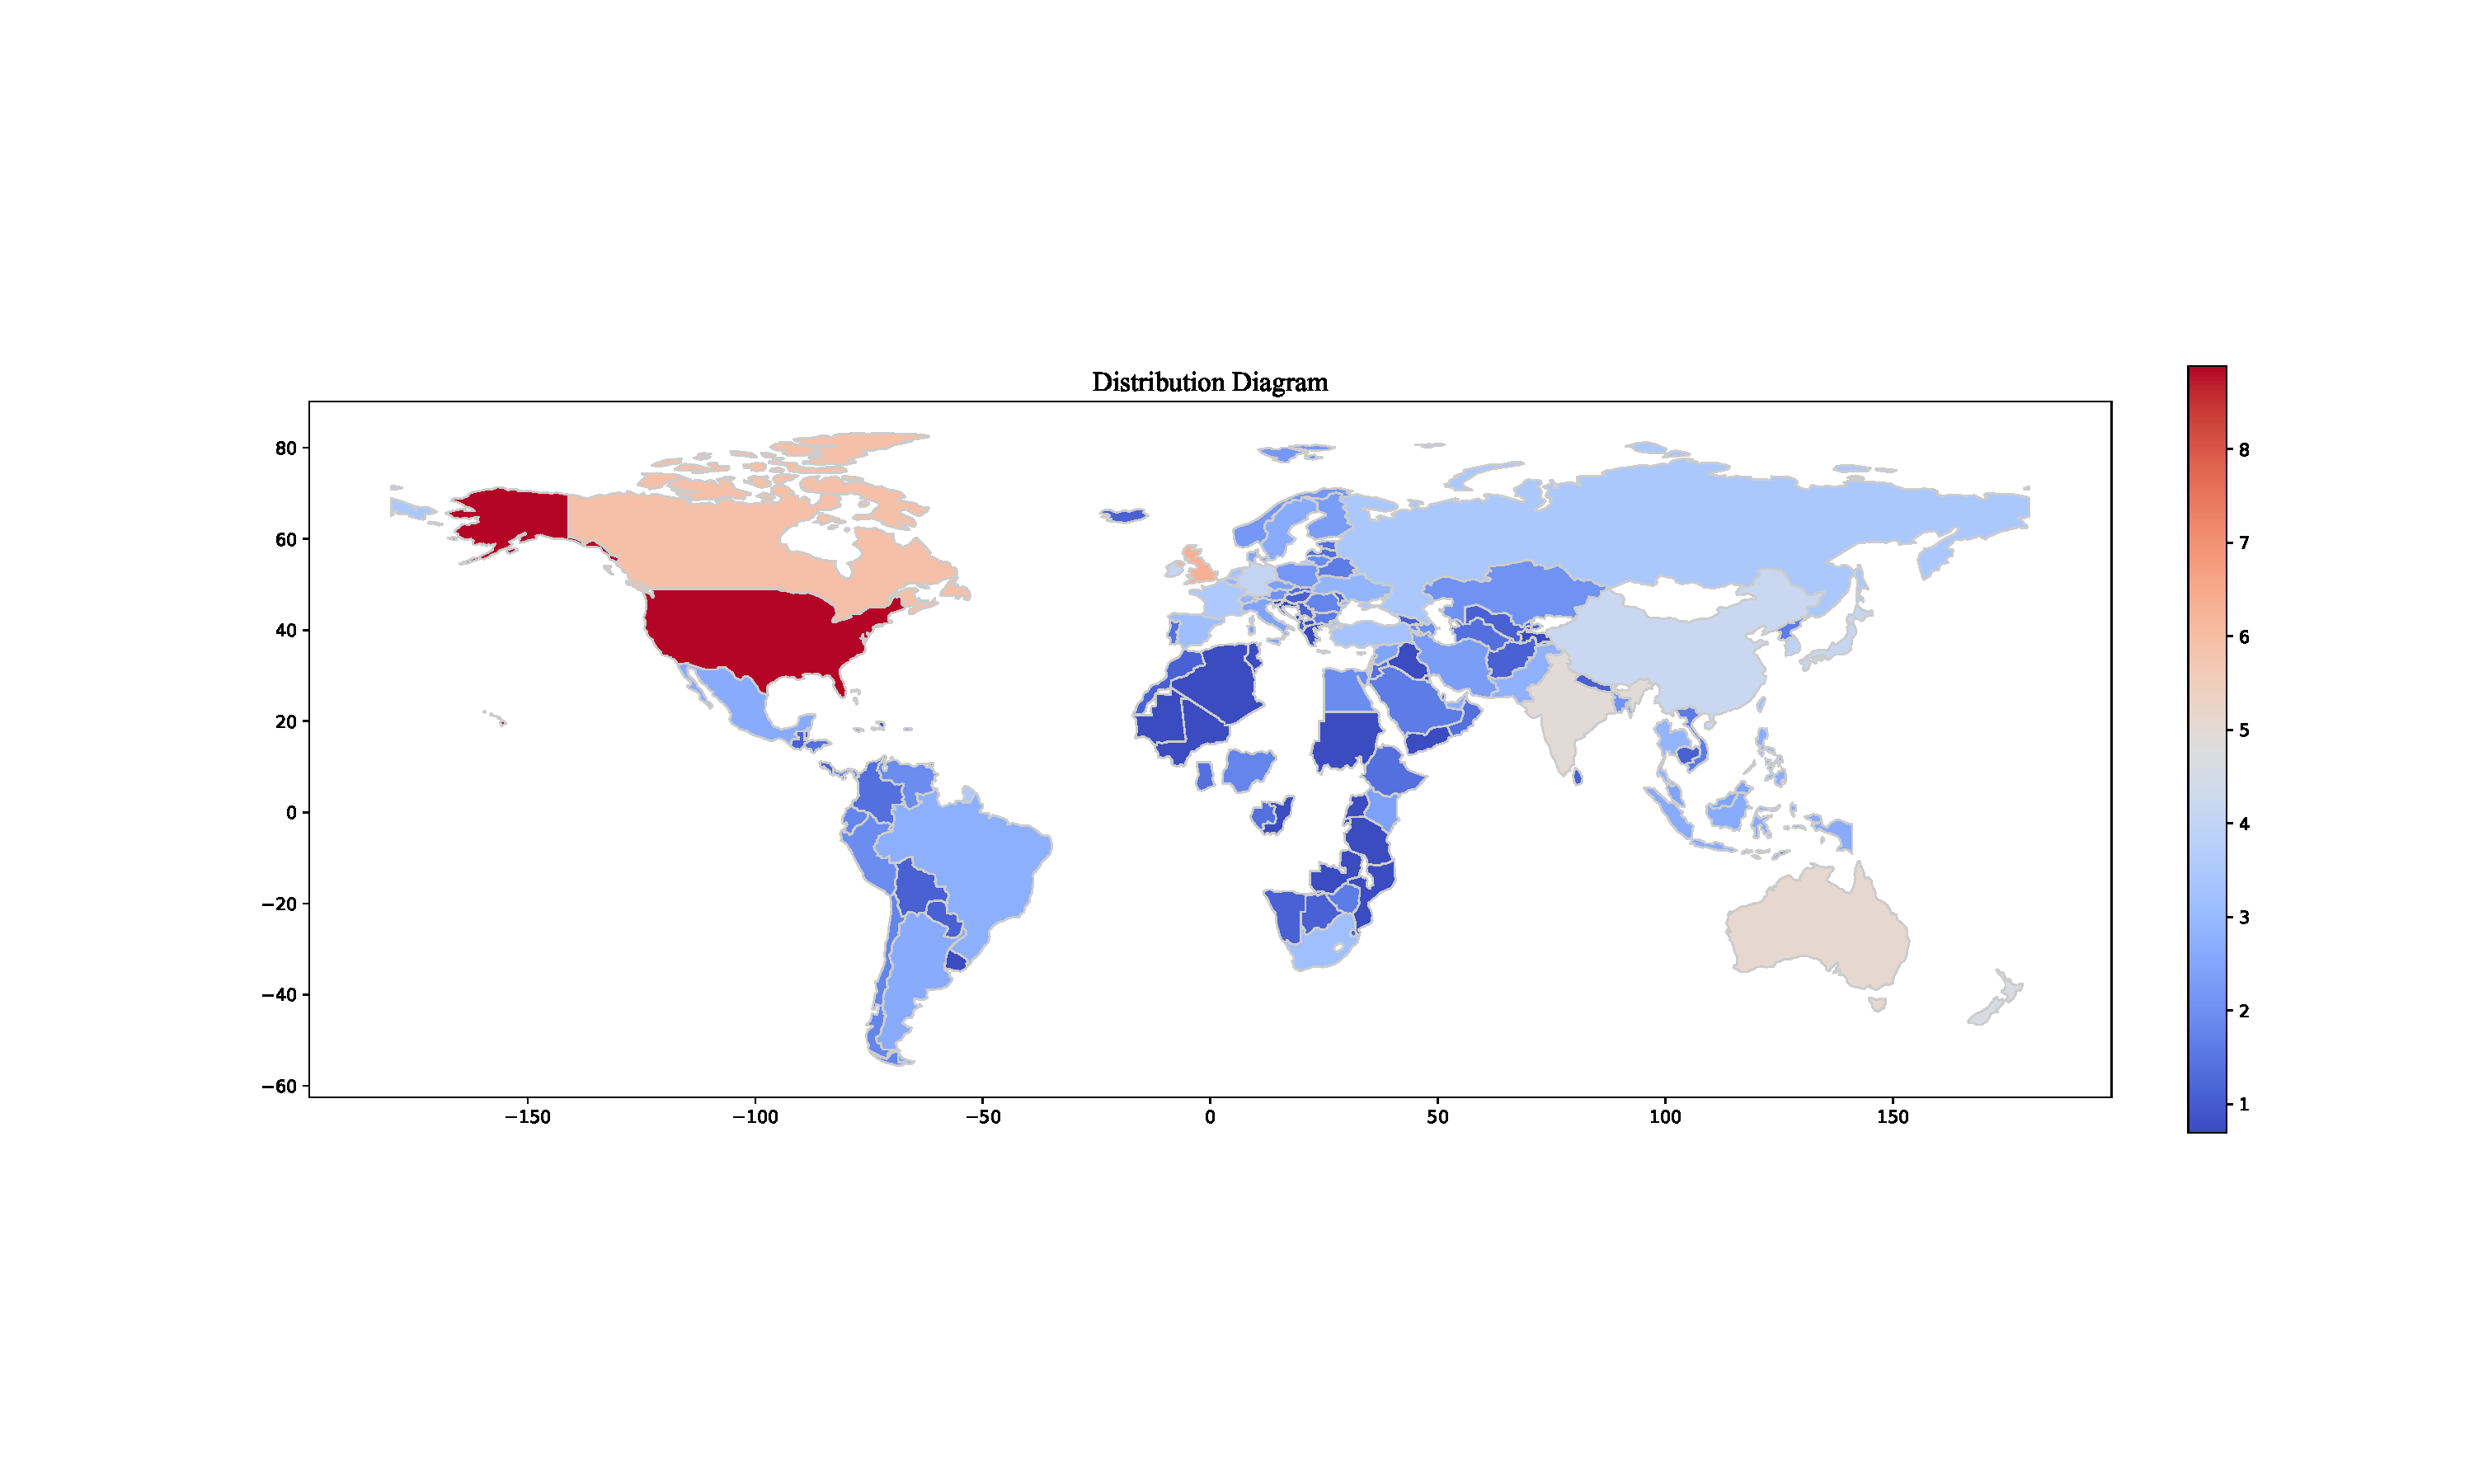
\includegraphics[width=1\linewidth]{../rsrc/distributions/Crime_distribution}
		\caption{Crime distribution}\label{fig:crime-distribution}
	\end{figure}
\subsection{High-prevalence regions}\label{subsec:high-prevalence-regions} %3.2
	We obtained population data $P_i$ for various countries over recent decades from the World Bank Group's website\cite{population}.
	Simultaneously, we processed data from the VCDB to tabulate the annual number of cybercrime incidents $D_i$ for each country from 2000 to 2025.
	However, due to discrepancies in the specific countries reported by the World Bank Group and those listed in the VCDB,
	we had to exclude certain countries to ensure that only those appearing in both datasets were retained.
	Ultimately, 109 countries were included in the model.
	To represent the average number of cybercrime incidents per capita,
	we calculated the ratio $D_i/P_i$ for each year from 2000 to 2025.
	Since the resulting values were too small for practical analysis,
	we scaled them by a factor of $10^{8}$ to express the data as the number of cybercrime incidents per 100 million people,
	denoted as $hmD/P_i$:
	\[ hmD/P_i = \frac{D_i}{P_i} \times 10^{8} \]

	According to the GCI (Global Cybersecurity Index) standards, countries are classified into five tiers, denoted as T1 to T5.
	We used this classification as the basis for K-means clustering analysis,
	dividing the 109 countries into five groups based on the percentiles published on the GCI website:
	the top 10\%, the next 20\%, the following 25\%, the subsequent 25\%, and the bottom 20\%.
	For each group, the annual average of $hmD/P_i$ (the number of cybercrime incidents per 100 million people) was calculated.
	To visualize the results, we constructed a 3D clustering heatmap of cybercrime trends,
	where the x-axis represents the five tiers (T1 to T5),
	the y-axis represents the time span from 2000 to 2025,
	and the z-axis represents the average $hmD/P_i$ values.
	This visualization is presented in Figure\ref{fig:3D_with_Spaced_Projection}.
	\begin{figure}[htbp]
		\centering
		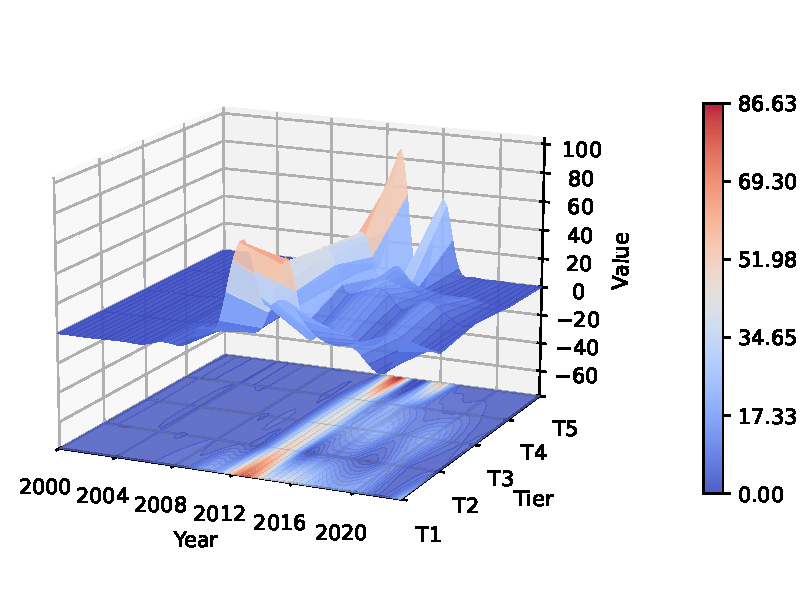
\includegraphics[width=0.75\linewidth]{../rsrc/distributions/3D_with_Spaced_Projection}
		\caption{3D with Spaced Projection}\label{fig:3D_with_Spaced_Projection}
	\end{figure}
\subsection{Other Cybercrime Incidents}\label{subsec:other-cybercrime-incedents} % 3.3
	Using additional data obtained from the VCDB,
	we constructed heatmaps on a global scale based on the number of successful cybercrimes, thwarted cybercrimes, and reported cybercrimes, respectively.
	Due to the disproportionately high volume of data from the United States,
	we applied the same logarithmic transformation (\( y = \log(1 + x) \)) as in Figure~\ref{fig:crime-distribution} for consistency,
	where $x$ represents successful attacks, thwarted attacks, and reported attacks,
	resulting in the three sub-figures presented in Figure\ref{fig:other-cybercrime-incidents}.

	In sub-figure (a), the number of successful attacks closely aligns with the total number of attacks in most countries.
	For instance, the United States recorded 7,189 successful attacks out of 7,236 total attacks,
	yielding a success rate of \( \frac{7189}{7236} \approx 99.35\% \).
	Similarly, the United Kingdom reported 569 successful attacks out of 574 total attacks,
	with a success rate of \( \frac{569}{574} \approx 99.13\% \).

	In contrast, countries with lower attack volumes did not show significant differences between the total number of attacks and the number of successful attacks,
	indicating that almost every attempted attack was successful.

	In sub-figure (b), only the United States and Canada reported thwarted attack cases, with 6 and 2 instances, respectively.

	In sub-figure (c), the number of successfully reported attacks and the number of countries involved were significantly higher than in sub-figure (b).
	This suggests that while many attacks were successful, a portion of them were detected and reported.
	\begin{figure}[htbp]
		\centering
		\subfloat[Successful Cybercrime Incidents]{
			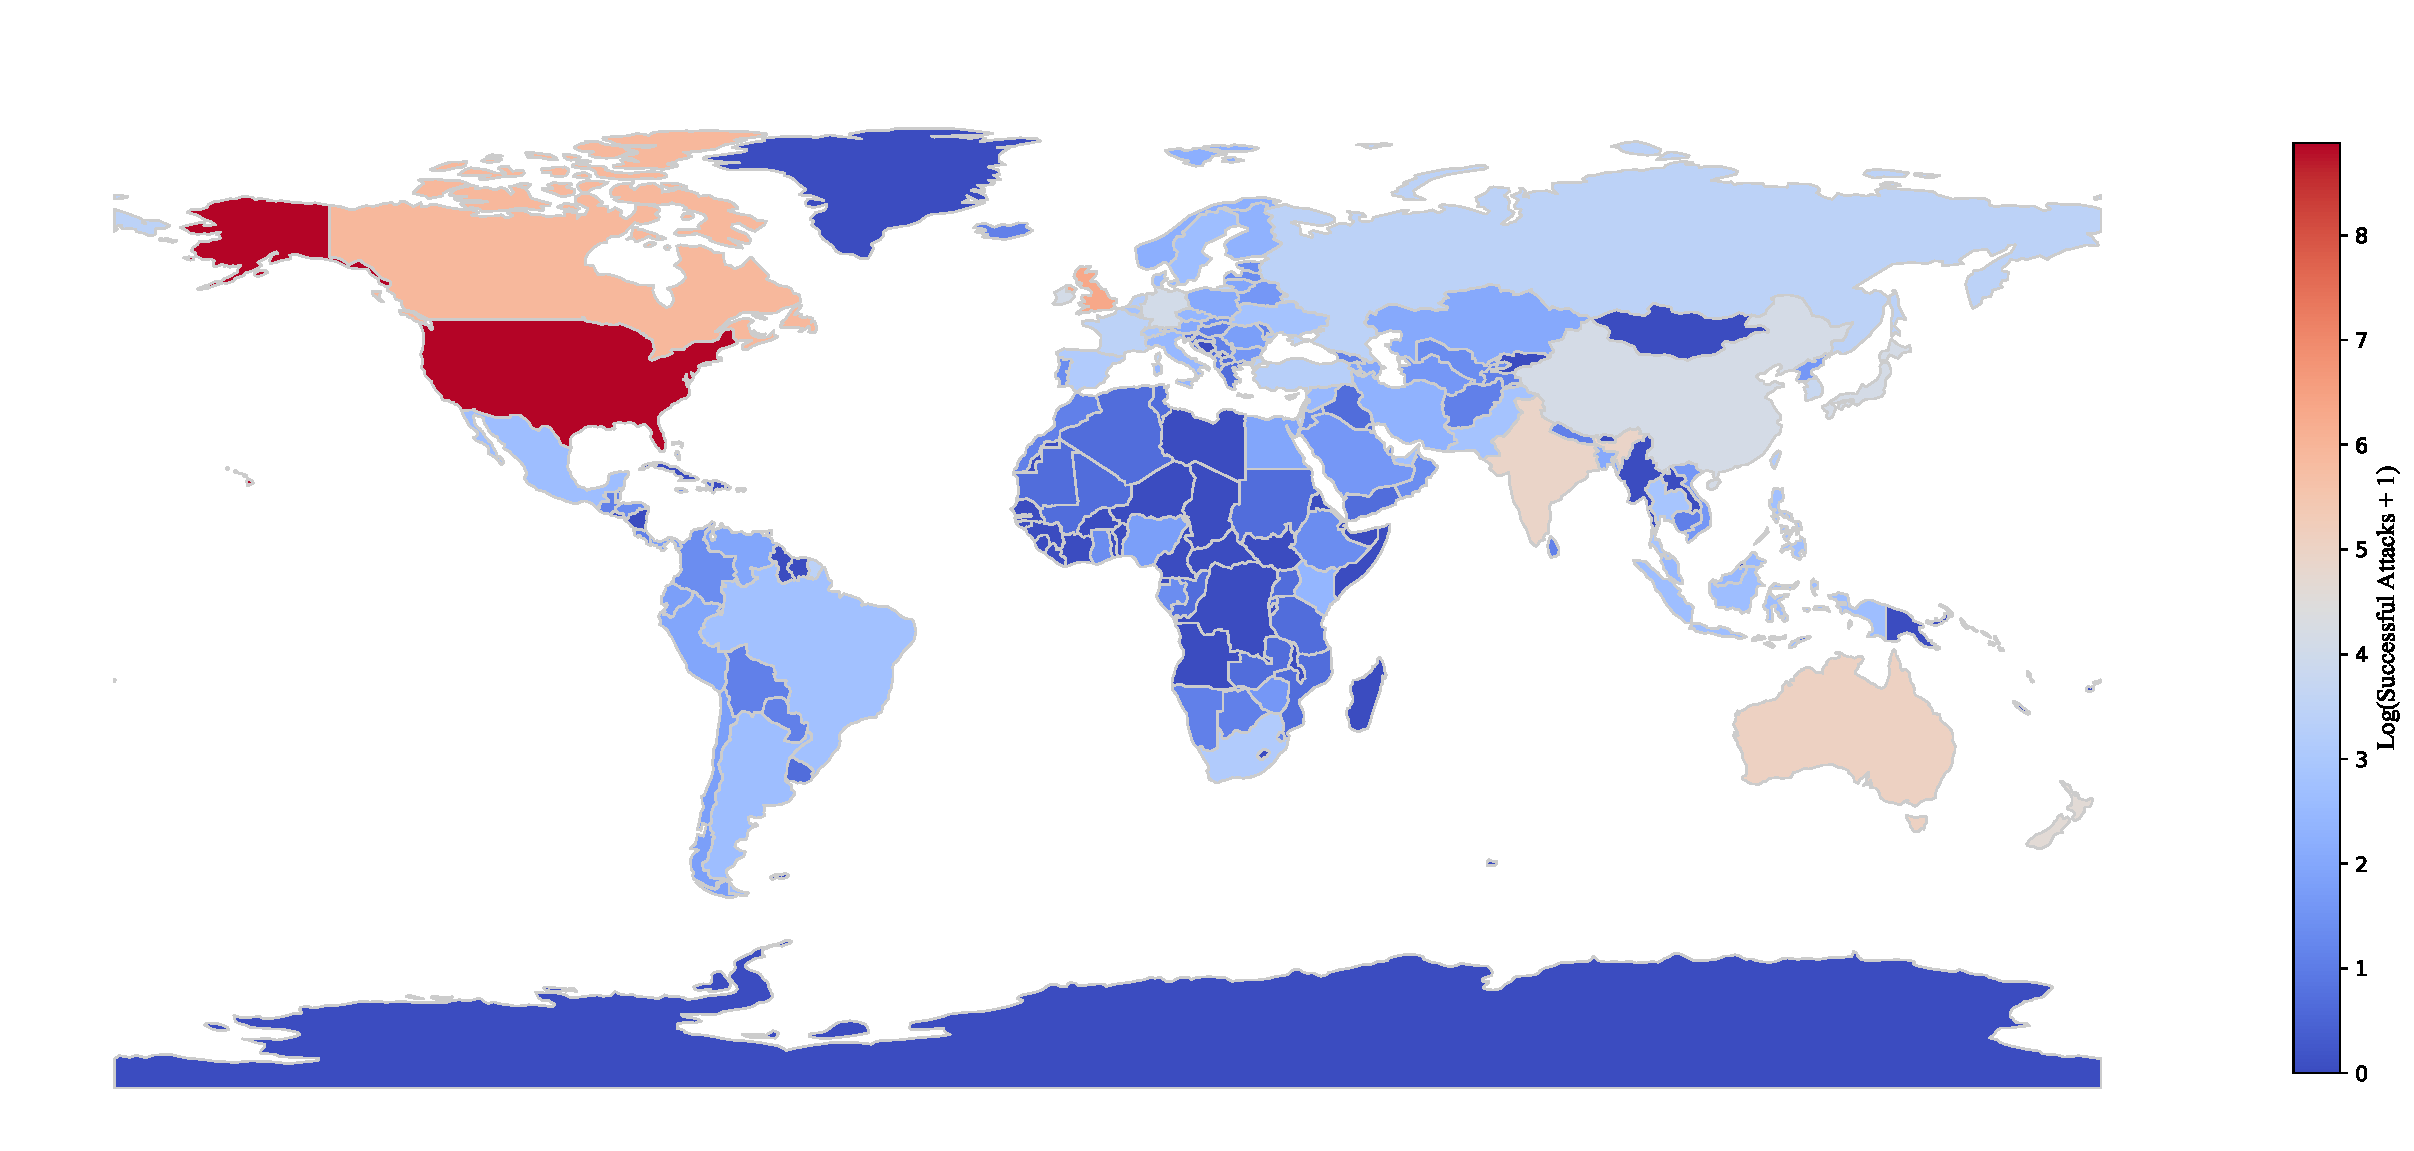
\includegraphics[width=0.8\linewidth]{../rsrc/distributions/Crime_Successful_distribution}
		}\\
		\subfloat[Mitigated Cybercrime Attempts]{
			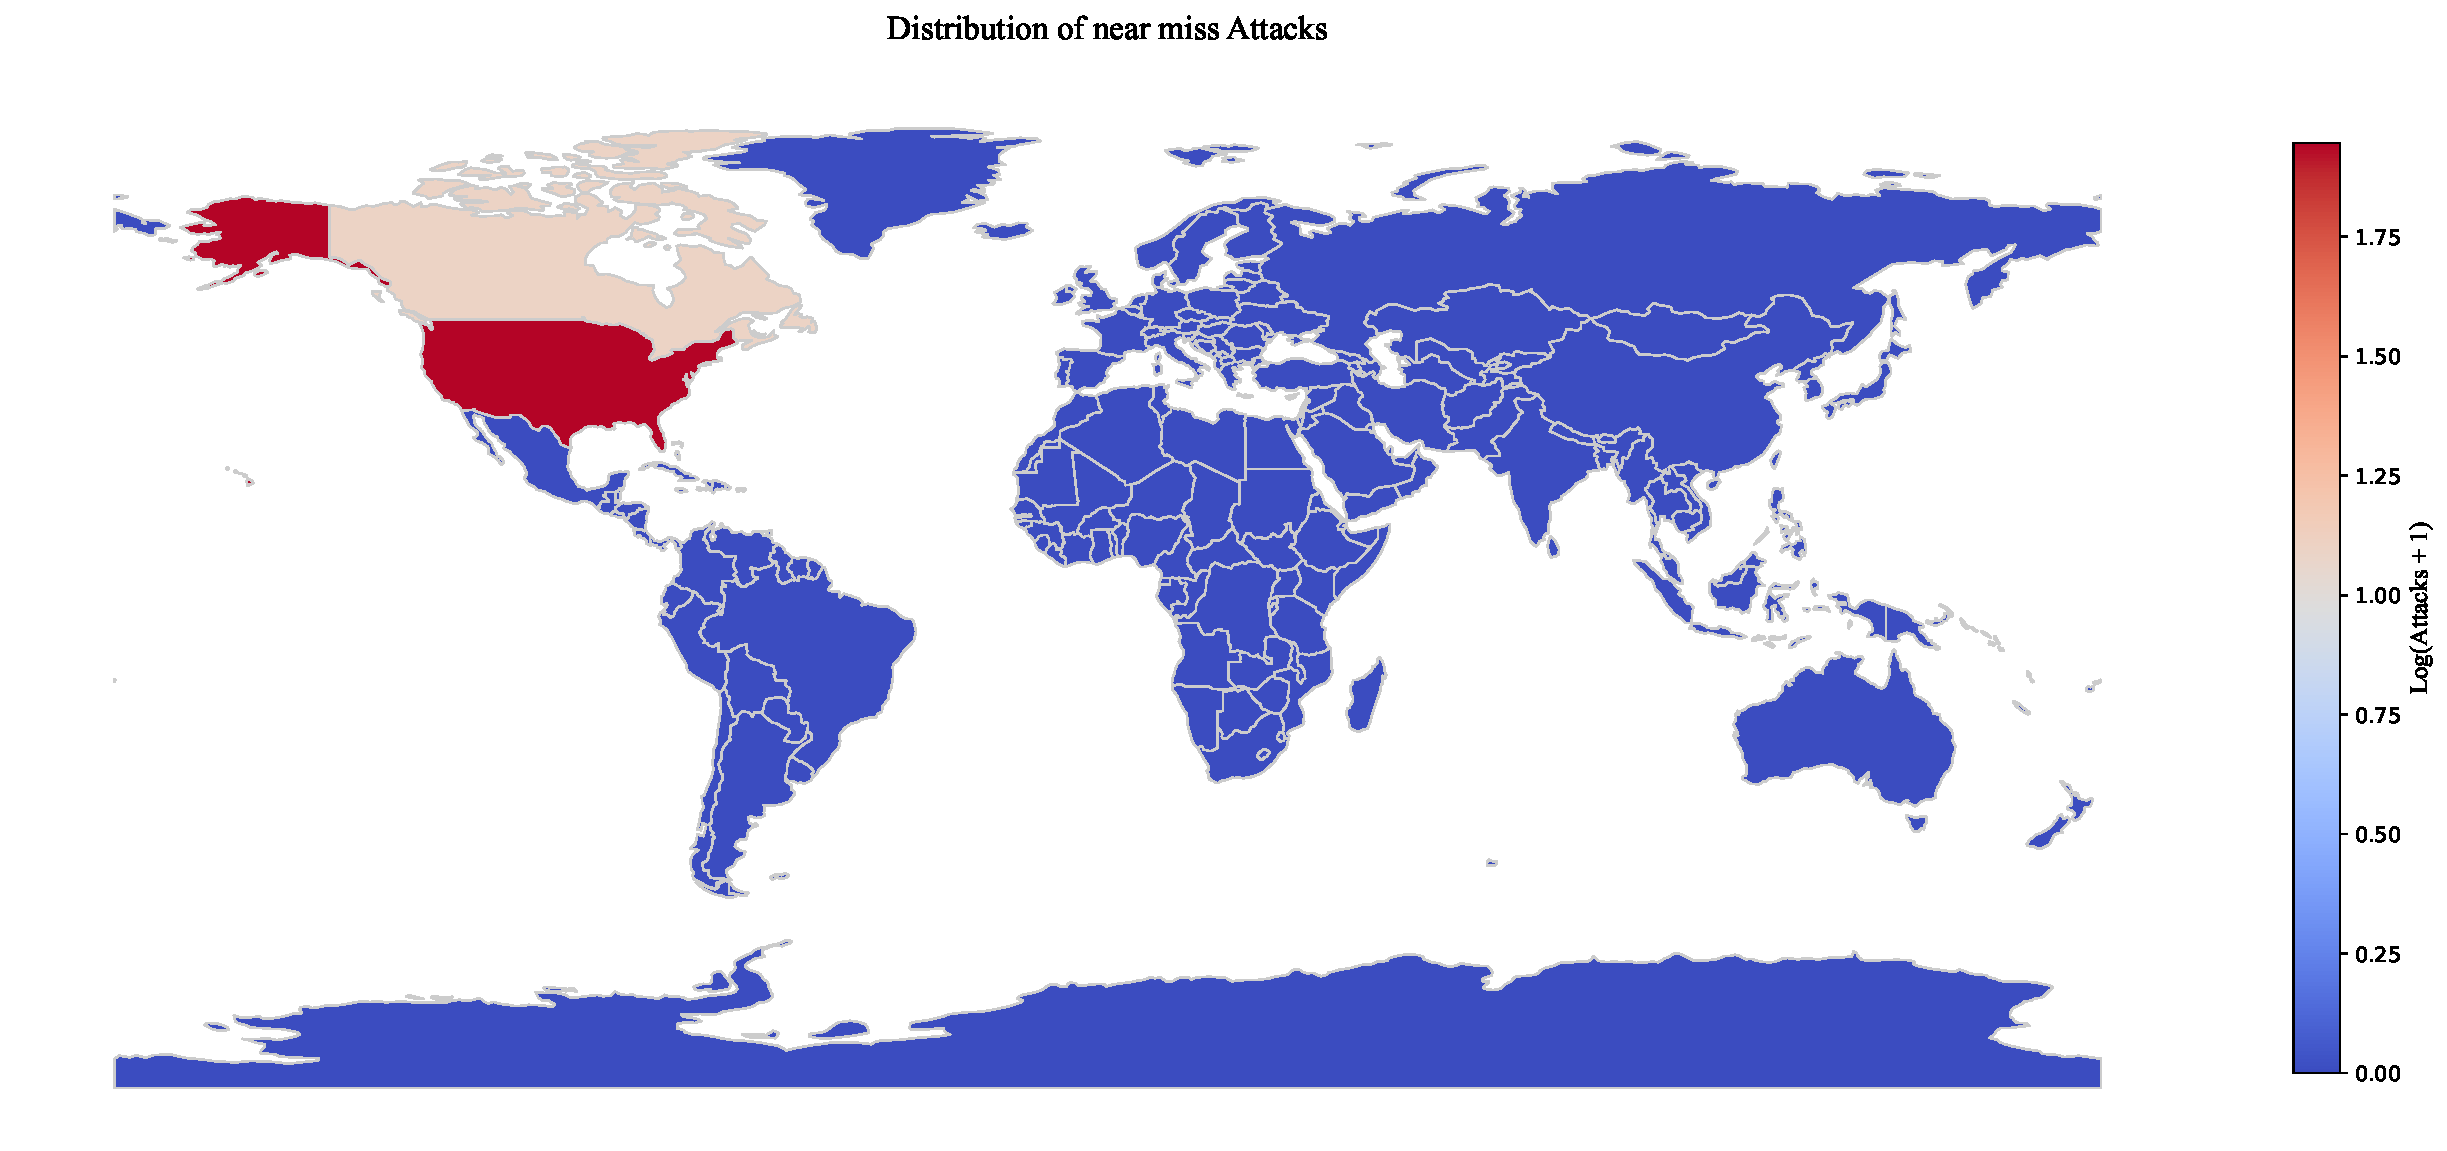
\includegraphics[width=0.4\linewidth]{../rsrc/distributions/Crime_NearMiss_distribution}
		}\hfill
		\subfloat[Reported Cybercrime Incidents]{
			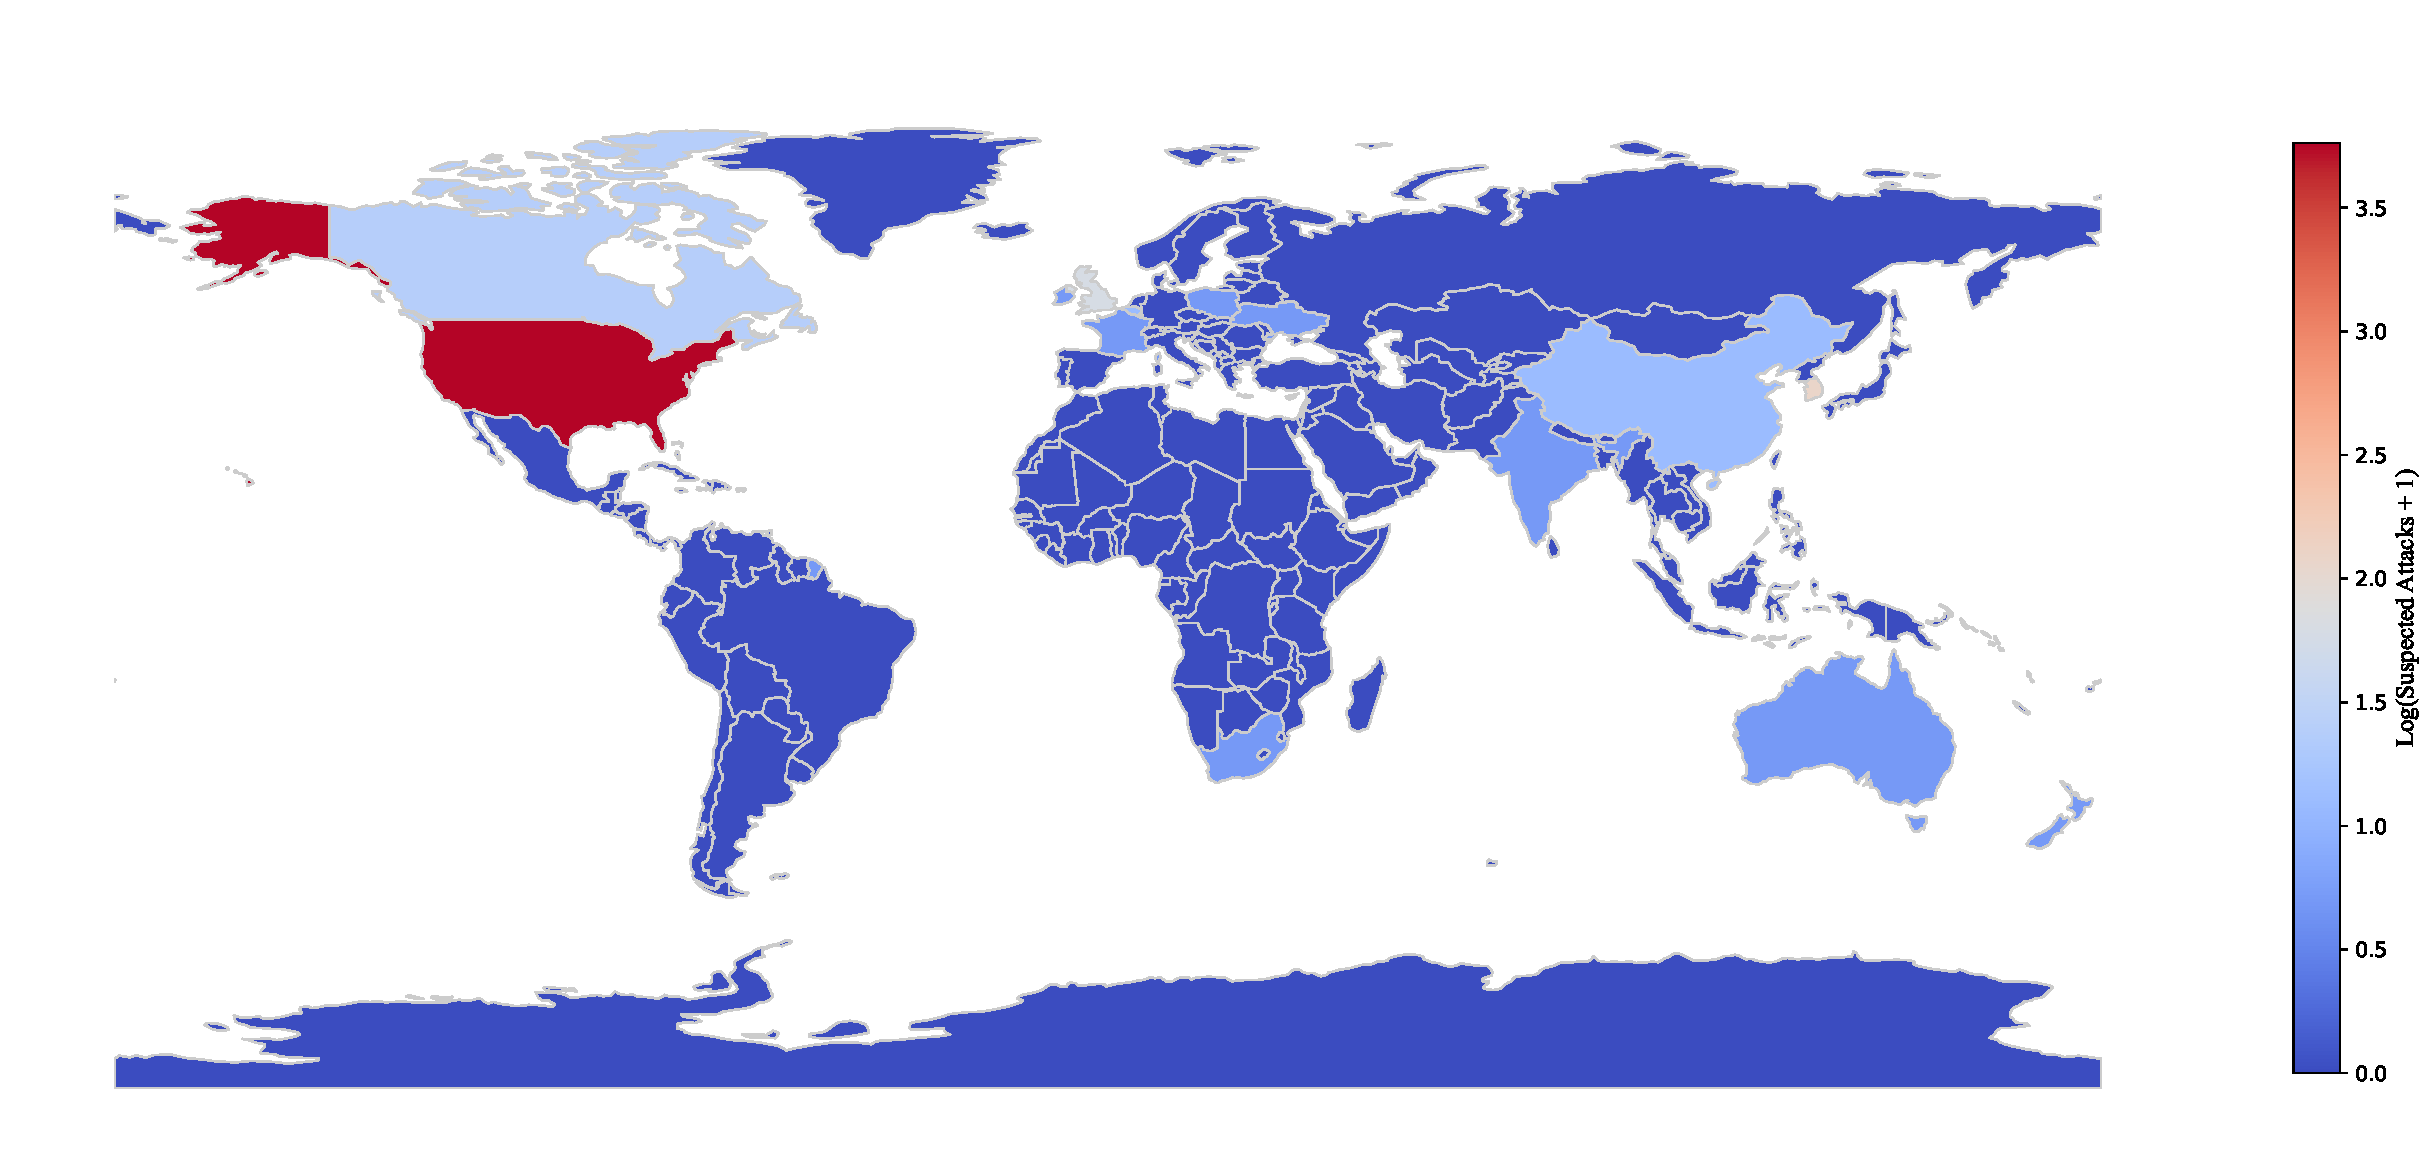
\includegraphics[width=0.4\linewidth]{../rsrc/distributions/Crime_Suspected_distribution}
		}\\
		\caption{Other Cybercrime Incidents}\label{fig:other-cybercrime-incidents}
	\end{figure}
\subsection{Pattern Discovery}\label{subsec:pattern-discovery} %3.4
	As shown in Figure~\ref{fig:other-cybercrime-incidents}, global cybersecurity capabilities remain unevenly distributed.
	The United States and Canada are the only countries with documented successful cyberattack defenses (6 and 2 cases, respectively),
	attributable to their mature cybersecurity ecosystems, technological investments, and high incident volumes that enable iterative defense refinement.
	Other nations lack comparable infrastructure or incident exposure, resulting in no reported defenses in the VCDB .

	Cybercrime trends across GCI tiers (T1-T5) reveal distinct spatio-temporal patterns (see Figure 2).
	From 2000 to 2025:

	\textbf{2012–2016}: T5 (lowest GCI tier) and T1 (highest tier) countries exhibited peak cybercrime activity.
	T5 nations reached a 25-year high ($hmD/P_i = 86.63$), driven by systemic deficiencies in legal, technical, and cooperative capacities.
	Conversely, T1 countries faced escalating threats despite high GCI rankings, reflecting unpreparedness for rapidly evolving cyber risks.

	\textbf{2016–2020}: Cybercrime declined globally,
	with T1 nations achieving the sharpest reductions through advanced infrastructure upgrades, stricter regulations, and international collaborations (e.g., VERIS data sharing).
	However, T5 countries remained disproportionately vulnerable due to persistent GCI metric weaknesses.

	\textbf{2020–Present}: T5 and T4 countries report near-zero cybercrime incidents—a paradoxical trend potentially linked to underreporting.
	Meanwhile, T1-T3 nations show sustained declines, likely reflecting cumulative gains from sustained cybersecurity investments.
	The abrupt T5 anomaly warrants further investigation into data transparency and measurement biases.